\documentclass[10pt]{beamer}

\mode<presentation> 
{
  \usetheme{Diku}
  \beamertemplatenavigationsymbolsempty
  \setbeamercovered{invisible}
%  \setbeamercovered{transparent}
}


% { \usetheme[nat,dogma]{Frederiksberg} }
%{ \usetheme[nat]{Frederiksberg} }

% \usepackage[danish]{babel}
\usepackage[latin1]{inputenc}
\usepackage{times,pslatex}
\usepackage[T1]{fontenc}
\usepackage[english]{babel}
\usepackage{hyperref}

\usepackage{multimedia}
\usepackage{francois-preamble}
\usepackage{multirow}
% \usepackage{multimedia}


\newcommand{\cc}{{c\!\!,}}
\newcommand{\degr}[1]{{{#1}^\circ}}
\DeclareMathOperator{\idf}{idf}

\title{Content Based Image Retrieval 2}

\author[S. Olsen] % (optional, use only with lots of authors)
{S�ren I. Olsen}
% Copied from Francois Lauze

\institute[DIKU] % (optional, but mostly needed)
{
  Department of Computer Science\\
  University of Copenhagen
}

\date[2014 B2] % (optional, should be abbreviation of conference name)
% {Research Presentation, Diku 2006}

% Insert page numbers
\pagenumbering{arabic}
\setbeamertemplate{footline}{\hspace{5pt}\insertpagenumber\vspace{10pt}}

\definecolor{gold}{rgb}{0.95,0.83,0.0}
\definecolor{orange}{rgb}{0.95,0.7,0.0}
% \definecolor{backblue}{rgb}{0.93,0.94,0.99}
\definecolor{backblue}{rgb}{0.95,0.94,0.99}
\setbeamercolor*{background canvas}{bg=backblue} 



\newcommand{\myemph}[1]{{\color{blue}{#1}}}
\newcommand{\intrg}[1]{\int_{{#1}=-\infty}^\infty}
\newcommand{\intRR}{\int_{-\infty}^\infty}

\AtBeginSection[]
{
  \begin{frame}<beamer>{Outline}
    \tableofcontents[currentsection,currentsubsection]
  \end{frame}
}


\begin{document}
\maketitle

% would be cool with more images showing applications


%-------------------------------------------------------------------
%   Start slides
%-------------------------------------------------------------------


%-------------------------------------------------------------------
\begin{frame}
  \frametitle{Assignment - details}
  \begin{itemize}
  \item The assignment consists in implementing a prototypical Content
    Based Image Retrieval System \\[5mm]
  \item Four parts:
    \begin{enumerate}
      \item Gather descriptors in training image data set \\[3mm]
      \item Construct codebook using k-means and Bag-Of-Words \\[3mm]
      \item Project test images onto codebook, and generate BoW \\[3mm]
      \item Retrieve according to similarity measure
    \end{enumerate}
  \end{itemize}
\end{frame}

%-------------------------------------------------------------------
\begin{frame}
\frametitle{What descriptors}
  \begin{itemize}
     \item   You are advised to use SIFT features
     \item   Few versions of SIFT include color. You may miss a lot of
       information. 
     \item   Color histograms etc.
     \item   Other descriptors: Texture
     \item   Advise: Keep it simple
  \end{itemize}
\end{frame}

%-------------------------------------------------------------------
\begin{frame}
  \frametitle{Training and testing}
  \begin{itemize}
    \item Split data into two parts. Don't look at the test data before
      testing \\[5mm]
    \item During development you may split the training data into a
      construction part and an evaluation part \\[5mm]
    \item Never use the test set for tuning ! \\[5mm]
    \item Download Caltech-101 image database (131 MB) with 101
      categories or the newer Caltech-256 base (1.2 GB)
  \end{itemize}
\end{frame}


%-------------------------------------------------------------------
\begin{frame}
  \frametitle{Data enough?}
  \begin{itemize}
    % \item One SIFT-key takes $2^{7+2}$ bytes. 
    \item Say we use 1000 clusters and need about 1000  
      elements per cluster, in total about 1M features for training. \\[3mm]
    \item The image size (of Caltech-101) is about $200 \times 300$
      generating on average about 1 percent key points [decriptors],
      say 1000. \\[3mm]  
%    \item To reach the needed amount af data for training we need at
%      least 1000 images (in practice more).
    \item The Calatech 101 base  has 101 categories with 40-800
      images/category, in total  9450 images.\\[3mm]
    \item {\color{red}{Exercise: Discuss with your neighbor: How many
          images/category can you save for testing ?}}
  \end{itemize}
\end{frame}

%-------------------------------------------------------------------
\begin{frame}
% \frametitle{What then?}
  \begin{itemize}
    \item {\color{red}{Exercise: Discuss with your neighbor: How many
          images/category can you save for testing ?}} \\[3mm]
    \pause
      On average, 9450 images provides about 10M SIFT-descriptors. We need 
      1M for training leaving 9M (or 90\%) for testing. We have plenty
      of data. \\[3mm]
    \item {\color{red}{What if we only have 20 images in one category
          and these images only generate 500 decriptors each ?}} \\[3mm]
      \pause
      Difficult to say, because we don't know if the images would
      generate new clusters. \\
    \item In general, we often want more data to make sure that it
      spans the complete range of possibilities.  
  \end{itemize}
\end{frame}




%-------------------------------------------------------------------
\begin{frame}
  \frametitle{What error ?}
  \begin{itemize}
    \item Error on training data versus error on test data \\[5mm]
    \item {\color{red}{Exercise: Explain what is the problem when
      the training error is less than the test error? }} \\[5mm]
    \pause
    \item Overfitting is a serious problem.  Often caused by using too
      few training data (or too complicated model) \\[5mm]
    \item We want to generalize in order to retrieve/classify new data
  \end{itemize}
\end{frame}



%-------------------------------------------------------------------
\begin{frame}
\frametitle{Which K ?}
  \begin{itemize}
    \item Most algorithms for clustering assumes K known \\[2mm]
    \item For very low-dimensional data visual exploration techniques
      (eg. plot3($\cdot$) in Matlab) may be used to guess K \\[2mm]
    \item For high-dimensional data an optimal choice is difficult to
      guess \\[2mm]
    \item K too small $\Longrightarrow$ Cannot model data \\[2mm]
    \item K too large $\Longrightarrow$ Overfitting \\[2mm]
    \item Problem: Often the average training error decreases 
      smoothly with K (no sudden decrease)
  \end{itemize}
\end{frame}



%-------------------------------------------------------------------
\begin{frame}
  \frametitle{Cross-validation}
  \begin{itemize}
    \item Divide data into say 10 sets (10-fold CV) \\[5mm]
    \item Train on all but one set that is used testing \\[5mm]
    \item Retrain and test on all possible combinations \\[5mm]
    \item Compute the average test error
  \end{itemize}
\end{frame}


%-------------------------------------------------------------------
\begin{frame}
  \frametitle{How to report}
  \begin{itemize}
    \item Amount: 5 pages including everything: 
      Try to be concise, structured etc. \\[5mm]
    \item Discussion: This is the most important part \\[5mm]
    \item Tables: Remember to tell me what I should notice \\[5mm]
    \item Figures: Remember axis labels etc.  What should I see? \\[5mm]
    \item Images: Don't show them too small. What should I see? \\[5mm]
    \item Explanations: Don't expect me to guess what you mean or see yourself
  \end{itemize}
\end{frame}


%-------------------------------------------------------------------
\begin{frame}
%   \frametitle{Questions}
%    $\mbox{}$ \\[16mm]

\begin{center}
  {\Huge {\color{blue}{QUESTIONS}}}
\end{center}
\end{frame}





%----------------------------------------------
\begin{frame}
  \frametitle{For the rest of today}
  \begin{itemize}
  \item Vectors and matrices.
  \item Linear algebra is probably the most important tool to solve
    real life (mathematical) problems.
  \item 3D reconstructions from projections is all (well almost) about
    Linear Algebra 
  \item If you are not a mathematician, please read the L.A.-turorial,
    its far from complete but gives a good start.
 \end{itemize}
\end{frame}



% ----------------------------------------------------
\begin{frame}
  \frametitle{Vectors}
  \begin{itemize}
  \item A $n$-vector is a $n$-tuple of real values:
    $$
    v =
    \begin{pmatrix}
      x_1\\\dots\\x_n
    \end{pmatrix}
    $$
  \item Addition
    $$
    \begin{pmatrix}
      x_1\\\vdots\\x_n
    \end{pmatrix}
    +
    \begin{pmatrix}
      y_1\\\vdots\\y_n
    \end{pmatrix}
    =
    \begin{pmatrix}
      x_1+y_1\\\vdots\\x_n+y_n
    \end{pmatrix}
    $$
  \item Multiplication by a scalar
    $$
    \lambda\begin{pmatrix}
      x_1\\\vdots\\x_n
    \end{pmatrix}
    = 
    \begin{pmatrix}
      \lambda x_1\\\vdots\\\lambda x_n
    \end{pmatrix}
    $$
  \end{itemize}
\end{frame}


% ----------------------------------------------------
\begin{frame}
  \frametitle{Linear Mapping}
  \begin{itemize}
   \item $f(v+ \lambda v') = f(v) + \lambda f(v')$
  \item Mapping between vectors with only addition of coordinates, multiplications by scalar and no constant terms.
  \item Example
    $$
    f
    \begin{pmatrix}
      x\\y\\z
    \end{pmatrix}
    =
    \begin{pmatrix}
      x+3y\\z-2x
    \end{pmatrix}
    $$
  \item Non linear example
    $$g
    \begin{pmatrix}
      x\\y\\z
    \end{pmatrix}
    =
    \begin{pmatrix}
      x^2+3yz\\z-2x^2 + 1
    \end{pmatrix}
    $$
    There are powers and constant terms.
  \end{itemize}
\end{frame}


% ----------------------------------------------------
% \begin{frame}
%  \frametitle{Linearity}
%  \begin{itemize}
%  \item This means $f(v+ \lambda v') = f(v) + \lambda f(v')$
%    \begin{align*}
%     f\left(
%    \begin{pmatrix}
%      x\\y\\z
%    \end{pmatrix}+\lambda
%    \begin{pmatrix}
%      x'\\y'\\z'
%    \end{pmatrix}
%    \right)
%    &= f
%    \begin{pmatrix}
%      x+\lambda x'\\y+\lambda y'\\z+\lambda z'
%    \end{pmatrix}\\
%    &=
%    \begin{pmatrix}
%      x+\lambda x'+3(y+\lambda y')\\
%      z+\lambda z'-2(x+\lambda x')
%    \end{pmatrix}\\
%    &=
%    \begin{pmatrix}
%      x+3y\\
%      z-2x\\
%    \end{pmatrix}
%    +\lambda 
%    \begin{pmatrix}
%      x'+3y'\\
%      z'-2x'
%    \end{pmatrix}\\
%    &= f
%    \begin{pmatrix}
%      x\\y\\z
%    \end{pmatrix}
%    + \lambda f
%    \begin{pmatrix}
%      x'\\y'\\z'
%    \end{pmatrix}
%  \end{align*}
% \item $f$ is linear.
% \end{itemize}
% \end{frame}

% ----------------------------------------------------
\begin{frame}
\frametitle{Vector product and transpose}
  \begin{itemize}
    \item The transpose ${\bf x}^{\top}$ of a column vector 
      ${\bf x}$ is a row vector. \\[3mm]     
    \item The transpose ${\bf y}^{\top}$ of a row vector 
      ${\bf y}$ is a column vector. \\[3mm]
    \item The product ${\bf x}^{\top} {\bf y}$ of a row and a column
      vector is a scalar. \\[3mm]
    \item The product ${\bf x} \cdot {\bf y}^{\top}$ of a column and a row
      vector is a matrix (se later). \\[3mm]
    \item If ${\bf x} \cdot {\bf y} = 0$, then ${\bf x}$ and ${\bf y}$
      are orthogonal (in between angle is 90 degrees).
\end{itemize}
\end{frame}


% ----------------------------------------------------
\begin{frame}
  \frametitle{Unit vectors and bases}
  \begin{itemize}
    \item A unit vector has a length of one: $\sum_i x_i^2 = 1$ \\[2mm]
    \item The Euclidean space $R^n$ is {\bf spanned} by $n$ (possibly unit) vectors
    \item A base for $R^n$ is $n$ unit vectors $e_i$ such that: \\[2mm]
      $$
      e_i \cdot e_j \;=\; \left \{ 
        \begin{array}{l l}
          1 & \mbox{if $i = j$} \\
          0 & \mbox{otherwise}
        \end{array} \right.
      $$
    \item {\color{red}{Exercise: Give an example on a base for $R^3$}}\\[2mm]
    \pause
    $\left \{ (0,0,1), (0,1,0), (1,0,0) \right \}$\\[2mm]
    \item The Euclidean (2-)norm of a vector ${\bf x}$ is denoted 
      $||{\bf x}||$ or more precisely $||{\bf x}||_2$ and computed by:  
      ${\sqrt{\sum_i x_i^2}}$
    \end{itemize}
\end{frame}
  

% ----------------------------------------------------
\begin{frame}
\frametitle{Projections}
A projection of a vector ${\bf u}$ on another vector ${\bf v}$ is
given by:
$$
\mbox{proj({\bf v, u})} 
 \;=\; 
      \left (
%     The line below generates a latex error      
        {\bf v}^{T}   %\hat} 
             \cdot \frac{\bf u}   {||{\bf u}||} 
      \right )
      \cdot \frac{\bf u}{||{\bf u}||}
 \;=\;
  ||{\bf v}|| \cos (\angle ({\bf v,u})) \frac{\bf u}{||{\bf u}||}
$$
\begin{center}
    \includegraphics[width=0.6\textwidth]{MyImages/VectorProjection.jpg}
\end{center}
\end{frame}



% ----------------------------------------------------
\begin{frame}
  \frametitle{Matrices}
  \begin{itemize}
  \item A $n\times m$ matrix is an array of numbers with $n$ rows and $m$ columns
  \item A 2$\times 3$ matrix $F$
    $$
    F =
    \begin{pmatrix}
      1 & 3 & 0\\
      -2 & 0 & 1
    \end{pmatrix}
    $$
  \item 2 matrices \myemph{of the same size} can be added together: just add the entries:
    $$    
    \begin{pmatrix}
      1 & 3 & 0\\
      -2 & 0 & 1
    \end{pmatrix}+
    \begin{pmatrix}
      4 & -2 & 1\\
      7 & -3 & 0
    \end{pmatrix}
    =
    \text{ ? }
    $$
  \end{itemize}
\end{frame}



% ----------------------------------------------------
\begin{frame}
\frametitle{Vectors and matrices}
A matrix is a:
\begin{itemize}
   \item Stack of row vectors \\[2mm]
   \item Concatenation of column vectors \\[2mm]
   \item Linear transformation between vector spaces \\[2mm]
   \item Basis for a vector space \\[2mm]
   \item A 2D array of numbers 
\end{itemize}
\end{frame}



% ----------------------------------------------------
\begin{frame}
  \frametitle{Product of a Matrix and a Vector}
  \begin{itemize}
  \item A matrix of size $m\times n$ and a vector of length $m$ can be
    multiplied to form a vector of length $n$. 
  \item Formal rule:
    $$
    A =
    \begin{pmatrix}
      a_{11}&\dots& a_{1n}\\
      \vdots & \vdots & \vdots\\
      a_{m1}&\dots& a_{mn}\\
    \end{pmatrix},
    v =
    \begin{pmatrix}
      v_1\\\vdots\\ v_n
    \end{pmatrix}
    $$
    $$
    A v =
    \begin{pmatrix}
      a_{11} v_1 + a_{12}v_2 + \dots a_{1m} v_n\\
      a_{21} v_1 + a_{22}v_2 + \dots a_{2m} v_n\\
      \vdots\\
      a_{m1} v_1 + a_{m2}v_2 + \dots a_{mn} v_n\\
    \end{pmatrix}
    $$
    \item Each line of $A$ is multiplied in ``inner product way'' with $v$.
  \end{itemize}
\end{frame}


% ----------------------------------------------------
\begin{frame}
  \begin{itemize}
  \item Example: Compute the product of 
    $$
    A =
    \begin{pmatrix}
        1 & 3 & 0\\
      -2 & 0 & 1
    \end{pmatrix}\text{ and }
    v =
    \begin{pmatrix}
      x\\y\\z
    \end{pmatrix}
    $$
    \pause
  \item We get
    $$   
    f
    \begin{pmatrix}
      x\\y\\z
    \end{pmatrix}
    =
    \begin{pmatrix}
      x+3y\\-2x+z
    \end{pmatrix}=
    \begin{pmatrix}
      x+3y\\z-2x
    \end{pmatrix}
    $$
  \item Each linear mapping can be written that way. Often use the same notation for the matrix and the linear mapping.
  \end{itemize}
\end{frame}


% ----------------------------------------------------
\begin{frame}
  \frametitle{Matrices /linear mappings as geometric \\ transformations}. 
  \begin{columns}
    \column{0.5\textwidth}
    \begin{center}
    Projection  on $x-y$ plane
    \end{center}
    \column{0.5\textwidth}
    \includegraphics[width=\textwidth]{FIGURES/3dto2dproj}
  \end{columns}
  \begin{center}
    \includegraphics[width=0.9\textwidth]{FIGURES/simpletransforms}\\
    Rotation of angle $\theta$ \hfill anisotropic scaling \hfill ~~~~~~shear~~~~~~~~~~~
  \end{center}
\end{frame}


% ----------------------------------------------------
\begin{frame}
  \begin{itemize}
  \item projection $\RR^3\to\RR^2$
    $$
    F
    \begin{pmatrix}
      x \\y \\z
    \end{pmatrix}
    =
    \begin{pmatrix}
      x \\y
    \end{pmatrix},\quad F =
    \begin{pmatrix}
      1 & 0 & 0\\
      0 & 1 & 0\\
      0 & 0 & 0
    \end{pmatrix}
    $$
  \item Rotation of angle $\theta$ from $\RR^2\to\RR^2$:
    $$
    R_\theta
    \begin{pmatrix}
      x \\y
    \end{pmatrix}
    =
    \begin{pmatrix}
      x\cos\theta - y\sin\theta\\
      x\sin\theta + y\cos\theta
    \end{pmatrix},\quad
    R_\theta =
    \begin{pmatrix}
      \cos\theta & -\sin\theta\\
      \sin\theta & \cos\theta
    \end{pmatrix}
    $$
  \item Scaling by a factor $\alpha$ in $x$ and $\beta$ in $y$:
    $$
    S
    \begin{pmatrix}
     x\\y 
    \end{pmatrix}
    = 
    \begin{pmatrix}
      \alpha x\\
      \beta y
    \end{pmatrix},\quad
    S =
    \begin{pmatrix}
      \alpha & 0\\0 & \beta
    \end{pmatrix}
    $$
  \item Shear of the $y$-axis with  angle $\theta$:
    $$
    \Ss
    \begin{pmatrix}
      x\\y
    \end{pmatrix}
    =
    \begin{pmatrix}
      x + \sin\theta y\\
      y
    \end{pmatrix},\quad
    \Ss =
    \begin{pmatrix}
      1 &\sin\theta\\
      0 & 1
    \end{pmatrix}
    $$
  \end{itemize}
\end{frame}


% ----------------------------------------------------
\begin{frame}
  \frametitle{Product of Matrices}
  \begin{itemize}
  \item A matrix of size $m\times n$ and a matrix of size $n\times p$
    can be multiplied to produce a matrix of size $m\times p$.
  \item Algebraic rule: $a_{ij}$ entry $(i,j)$ of $A$, $b_{jk}$ entry $(j,k)$ of $B$
    $$
    A = (a_{ij})_{\substack{i=1\dots m\\j=1\dots n}},\quad 
    B = (b_{jk})_{\substack{j=1\dots n\\k=1\dots p}}
    $$
    Denote entry $(i,k)$ of product $C = AB$ by $c_{ik}$:
    $$
    c_{ik} = \sum_{j = 1}^n a_{ij}b_{jk}
    $$
  \item Matrix vector multiplication is in fact a special case of it!
  \item Example
    $$
    \begin{pmatrix}
      2 & 2\\
      1 & 3\\
      1 & -1\\
    \end{pmatrix}
    \begin{pmatrix}
      1 & 3 & 0\\
      -2 & 0 & 1
    \end{pmatrix}
    = \onslide<2->
    \begin{pmatrix}
      -2 & 6 & 2\\
      -5 & 3 & 3\\
      3 & 3 & -1
    \end{pmatrix}
    $$
  \item What does matrix multiplication means?
  \end{itemize}
\end{frame}


% ----------------------------------------------------
% \begin{frame}
%  \frametitle{Meaning of the Product}
%  \begin{itemize}
%  \item $M$ and $N$ the linear mappings $
%    \begin{pmatrix}
%      2 & 2\\
%      1 & 3\\
%      1 & -1\\
%    \end{pmatrix}
%    $ and 
%    $
%    \begin{pmatrix}
%      1 & 3 & 0\\
%      -2 & 0 & 1
%    \end{pmatrix}
%    $
%  \item
%    Apply $N$ to $
%    \bv = \begin{pmatrix}
%      x \\ y \\ z
%    \end{pmatrix}
%    $
%    and $M$ to get the result:
%    $$
%    N \bv = \begin{pmatrix}
%      1 & 3 & 0\\
%      -2 & 0 & 1
%    \end{pmatrix}\begin{pmatrix}
%      x \\ y \\ z
%    \end{pmatrix}
%    = 
%    \begin{pmatrix}
%      x + 3y\\
%      -2x + z
%    \end{pmatrix}
%    $$
%    \item and{\small
%      $$
%      \begin{pmatrix}
%      2 & 2\\
%      1 & 3\\
%      1 & -1\\
%    \end{pmatrix}
%     \begin{pmatrix}
%      x + 3y\\
%      -2x + z
%    \end{pmatrix}
%    =\onslide<2->
%    \begin{pmatrix}
%      -2x+6y+2z\\
%      -5x + 3y+3z\\
%      3x + 3y-z
%    \end{pmatrix}
%    =\onslide<3->
%    \begin{pmatrix}
%      -2 & 6 & 2\\
%      -5 & 3 & 3\\
%      3 & 3 & -1
%    \end{pmatrix}
%    \begin{pmatrix}
%      x\\y\\z
%    \end{pmatrix}
%    $$}
%    % \item VIP (Very Important Property) \myemph{Matrix multiplication corresponds to chaining linear transforms}!
%   \end{itemize}
% \end{frame}


% ----------------------------------------------------
\begin{frame}
\frametitle{Matrix multiplication is NOT commutative}
Please notice the $A B \;\neq \; B A$ \\[4mm]

{\color{red}{Exercise: Please calculate:}} 
\begin{displaymath}
   \left (
   \begin{array}{c c}
       1 & 4 \\
       0 & 2 
     \end{array}
   \right )
   \cdot
   \left (
   \begin{array}{c c}
       1 & 2 \\
       3 & 0 
     \end{array}
   \right )
   \hspace{4mm} \mbox{and} \hspace{4mm}
   \left (
    \begin{array}{c c}
       1 & 2 \\
       3 & 0 
     \end{array}
   \right )
   \cdot
   \left (
   \begin{array}{c c}
       1 & 4 \\
       0 & 2 
     \end{array}
  \right )
\end{displaymath}
\pause
Did you get:
\begin{displaymath}
   \left (
   \begin{array}{c c}
       13 & 2 \\
         6 & 0 
     \end{array}
   \right )
   \hspace{14mm} \mbox{and} \hspace{14mm}
   \left (
    \begin{array}{c c}
       1 & 8 \\
       3 & 12 
     \end{array}
   \right )
\end{displaymath}


\end{frame}


% ----------------------------------------------------
\begin{frame}
\frametitle{Rank, Linear independence}
  \begin{itemize}
    \item A set of vector are linear dependent if one of them may be
      constructed a a linear combination of the others, ie. if it is
      lying in the subspace spanned by the others. \\[3mm]
    \item The rank of a matrix is the maximal number of independent
      row (or column) vectors it is build of. \\[3mm]
    \item A matrix is called {\color{blue}{rank deficient}} or 
      {\color{red}{singular}} if is does
      not have full rank, ie. if there exist a linear dependence. \\[3mm]
    \item A rank-deficient matrix has no inverse
  \end{itemize}
\end{frame}






% ----------------------------------------------------
\begin{frame}
 \frametitle{Exercise}

{\color{red}{Is the following matrices rank deficient ?  What is the
    rank ?}} \\[3mm]
\begin{center}
$   
   \begin{pmatrix}
     -2 & 6 & 2\\
       1 &-3 & -1\\
       3 & -9 & -3
  \end{pmatrix}
$ \\[6mm]
$
   \begin{pmatrix}
     -2 & 6 & 2\\
     -5 & 3 & 3\\
       3 & 3 & -1
  \end{pmatrix}
$\\[6mm]
$
   \begin{pmatrix}
      1 & 0 & 1\\
      0 & 1 & 1\\
      7 & 3 & 0
  \end{pmatrix}
$
\end{center}
\end{frame}






% ----------------------------------------------------
\begin{frame}
  \frametitle{Matrix Product as Chain Application \\ of Linear Mappings}
  \begin{itemize}
  \item Matrix multiplication corresponds to chaining linear transforms:
    $$
    M\left (N\bv\right) = \udesc{\text{Matrix product}}{M N}\bv
    $$
  \item Very Important Property: Matrix product corresponds to chain application (composition) of linear mappings!
  \end{itemize}\vfill
  \begin{center}
    \large
    Read the Linear Algebra Tutorial and Reference on Absalon!   
  \end{center}
  This will also be useful for other courses!
\end{frame}


% ----------------------------------------------------
\begin{frame}
  \frametitle{Matrix transpose and inverse matrix}
  \begin{itemize}
   \item $K^\top$ is the transposed of $K$: inverse row and line indices.
     $$ 
     {\begin{pmatrix}
       h_{11} & h_{12} & h_{13} \\
       h_{21} & h_{22} & h_{23} \\
       h_{31} & h_{32} & h_{33} 
     \end{pmatrix}}^{\top}
     =
     \begin{pmatrix}
       h_{11} & h_{21} & h_{31} \\
       h_{12} & h_{22} & h_{32} \\
       h_{13} & h_{23} & h_{33} 
     \end{pmatrix}
     $$
   \item $K^{-1}$ is the inverse of a non-singular square
     matrix $K$. The inverse does not always exist. 
     $$
       y = Ax \implies x = A^{-1}y  
       \hspace{2mm} \mbox{and} \hspace{2mm}
       A A^{-1} = A^{-1}A = I
     $$
     where $I$ is the identity.
   \item $K^{-\top}$ means inverse of the transposed matrix: The same
     as transposed of the inverse.
   \end{itemize}
\end{frame}


% ----------------------------------------------------
\begin{frame}
\frametitle{Matrix equations}
Assume we have $n$ linear equations:
\begin{displaymath}
  a_{i1} x_1 \;+\; a_{i2} x_2 \;+\; \cdots \;+\; a_{im} x_m \;\; = \;\; b_i
\end{displaymath}
in $m$ unknowns $x_j$.  Then we may construct the $n \times m$
{\color{red}{Design matrix}} $A$ with elements $(a_{ij})$ and write the
matrix equation:
\begin{displaymath}
  A {\bf x} \;\;=\;\; {\bf b}
\end{displaymath}
 Since $A$ may not be square (hopefully $n \gg m$) we cannot invert
 $A$, but we may multiply by $A^{\top}$ and invert $A^{\top} A$
\begin{displaymath}
    {\bf x} \;\;=\;\; (A^{\top} A)^{-1}  A^{\top}{\bf b} \;\;=\;\; A^{\dagger} {\bf b}
\end{displaymath}
The matrix $A^{\dagger}$ is called {\color{red}{The pseudo inverse}}. In
practice there are more efficient ways to solve the matrix equation.
\end{frame}



% ----------------------------------------------------
\begin{frame}
\frametitle{Bilinear forms}
We shall later see non-linear relations between image projections
where we have products of coordinate values $(x_1, y_1)$ and $(x_2, y_2)$:

\begin{displaymath}
  f_1 x_1 x_2 + f_2 x_1 y_2 + f_3 x_1 +
  f_4 y_1 x_2 + f_5 y_1 y_2  + f_6 y_1 +
  f_7       x_2 + f_8       y_2  + f_9
  \;\; = \;\; 0
\end{displaymath}
If we organize the coefficients $(f_i)$ in a $3 \times 3$ matrix $F$
and let ${\bf x} = (x_1, y_1, 1)^{\top}$ and ${\bf x'} = (x_2, y_2, 1)^{\top}$
then we get:
\begin{displaymath}
  {\bf x}^{\top} F {\bf x'}  \;\;=\;\; 0
\end{displaymath}
We shall later see that this equation defines the {\bf Fundamental matrix}
which is central in {\color{red}{multi-view geometry}}.
\end{frame}




% ----------------------------------------------------
\begin{frame}
\frametitle{Matrix factorizations}
Matrices may be factorized (into products of other matrices) in a
number of ways: \\[3mm]
\begin{itemize}
  \item LU-decomposition
  \item Eigenvalue decomposition
  \item QR-decomposition
  \item SVD-decomposition \\[3mm]
\end{itemize}
You are not suposed to know these, nor their advantages etc, but they
are really usefull. We will later use the Singular Value Decomposition (SVD).

\end{frame}




% ----------------------------------------------------
\begin{frame}
\frametitle{Eigenvalues and eigenvectors}
The eigenvectors ${\bf e}_i$ and corresponding eigenvalues $\lambda_i$
of a square  matrix $A$ satisfies that:
\begin{displaymath}
  A {\bf e}_i  \;\;=\;\; \lambda_i {\bf e}_i
\end{displaymath}
It is easy to see that the eigenvalues are the roots of the
characteristic polynomium:
\begin{displaymath}
  \det (A  - \lambda I)  \;\;=\;\; 0
\end{displaymath}
If $Q$ is the matrix of stacked eigenvectors and $\Lambda$ is a
diagonal matrix of eigenvalues $\lambda_i$ it is also easy to see that:
\begin{displaymath}
   Q^{-1} A  Q  \;\;=\;\; \Lambda
\end{displaymath}
$Q$ is {\color{red}{diagonalizing}} $A$.  Eigenvalue analysis is
central in Image analysis and machine learning, eg. in Principal
component analysis and dimensionality reduction.
\end{frame}


\end{document}


